\documentclass[12pt,letterpaper]{article}
\usepackage{preamble}

\usepackage[utf8]{inputenc}
\usepackage[english]{babel}
\usepackage{listings}
\usepackage{mathtools}
\usepackage{amsmath}
\usepackage{enumitem}
\usepackage{csvsimple}
\usepackage{booktabs}

\lstdefinelanguage{alg}{
morekeywords={def,if,then,else,while,do,assert,end}
}


\newcommand\course{CSE 625}
\newcommand\hwnumber{1}
\newcommand\userID{Max Williams}

\newcommand{\tf}[2]{\frac{\text{#1}}{\text{#2}}}

\newcommand{\problem}[1]{\textit{#1} \medskip}
\newcommand{\solution}{ \noindent \textbf{Solution:} \medskip}

\begin{document}

\section*{Problem 1}

\problem{Given 64 elements in an array in shared memory and 8 PEs, design an efficient parallel
computing algorithm to compute the sum. Assuming it takes 1 second to add two numbers and 2 seconds
to read or write a number, describe your design and calculate the total time required to compute the
sum.}

\solution

First, divide the array into 8 sub-arrays with 8 numbers each. Each PE adds elements 0-7 to a local
varible \lstinline{total}, then write that value back to index 0 of its sub array.
This creates 8 values that can be added in
a merge as follows: $PE_0$ to $PE_3$ add up elements at index pairs (0, 8), (16, 24), (32, 40), and 
(48, 56), putting the result into the first index of the pair. Then $PE_0$ and $PE_1$ add up pairs 
(0, 16) and (32, 48), respectively. Then $PE_0$ adds values at 0 and 32, storing the result in 0,
completing the computation.

Python-ish pseudocode and timing analysis is given.

\lstinputlisting[language=Python,caption={p is the index of the processing element, from 0 to 7. It
is assumed that all thread are running in simultaneous lockstep so no synchonization is
needed.},captionpos=t]{problem1.alg}

Line 5 is called 8 times by each processor, and consists of one read (fetching the element from the
array) and one addition (adding to \lstinline{total}). This takes a total of $(2+1)\times 8 =$
\textbf{24 seconds} (8 compute, 16 memory). 
\lstinline{total} is stored in the start of each processor's subarray, which takes only one
write, \textbf{2 seconds} (0 compute, 2 memory). After half of the processors drop out, the
remaining four processors each add one element of the array to another and store the result in the
array, on line 12. This takes two reads, one addition, and one write, which takes 7 seconds. This is
repeated on line 17 and 22, for a total of \textbf{21 seconds} (3 compute, 18 memory).

In total, this gives 47 seconds to compute the sum. Only 11 of these are spent on additions, showing
the I/O bottleneck in distributed computing.

\section*{Problem 2}

\problem{Consider the Weak Scalability Analysis for $n = 1024\times p$ on slide 17.}

\subsection*{Problem 2.a}

\problem{Give the equations for Speedup and Efficiency in terms of $p$, respectively.}

In Equation \ref{eq:p2given}, we are given an equation for $T(2^q, 2^k)$. Since equations for speedup
and efficiency are given in terms of $T$ of $p$, we need to first find $T(p, n)$ then substitute in
for speedup and efficiency.

\begin{align} 
    T(p, n) &= T(2^q, 2^k) = 2^{k-q}-1+7q \label{eq:p2given}\\
    &p = 2^q\ \text{and}\ n = 2^k \nonumber\\
    &q = \log_2(p)\ \text{and}\ k = \log_2(n) \label{eq:qk}\\
    T(p, n) &= 2^{\log_2(n)-\log_2(p)}-1+7 \log_2(p) \nonumber\\
    T(p, n) &= \frac{n}{p}-1+7 \log_2(p) \label{eq:fort}
\end{align}

We can then find speedup:

\begin{equation} \label{eq:p2speedup}
    \text{Speedup} = \frac{T(1, 1024\times p)}{T(p, 1024\times p)} = \frac{1024\times p-1}{1023+7\log_2(p)}
\end{equation}

and efficiency:

\begin{equation} \label{eq:p2efficiency}
    \text{Efficiency} = \frac{\text{Speedup}}{p} = \frac{1024\times p-1}{p(1023+7\log_2(p))}
\end{equation}

\subsection*{Problem 2.b}

\problem{Define the equations of Speedup and Efficiency as R functions and verify the
Speedup and Efficiency values given on slide 17 using these R functions.}

\lstinputlisting[language=R,caption={R code to plot efficieny and speedup.},captionpos=t]{problem2.r}



\subsection*{Problem 2.c}

\problem{Use R to plot Speedup and Efficiency similar to those given on slide 17.}

See Figure \ref{fig:plot2} on page \pageref{fig:plot2}

\begin{figure}[h]
    \caption{Plots of speedup and efficiency.}
    \centering
    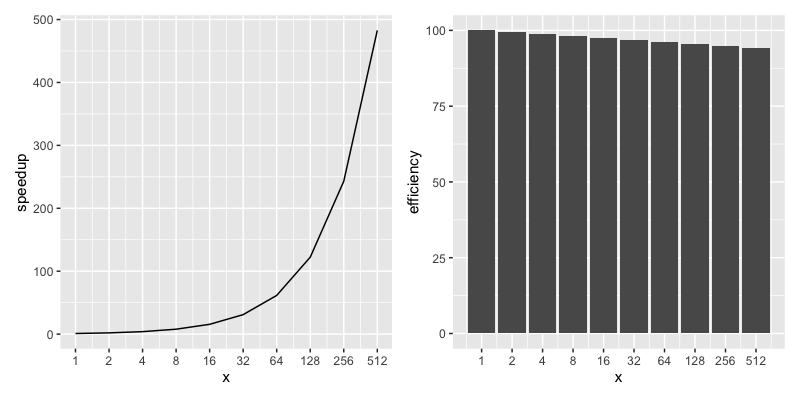
\includegraphics[width=7in]{plot2}
    \label{fig:plot2}
\end{figure}


\section*{Problem 3}

\problem{Consider slides 18-20 (the general case of computing sum using p PEs).}

\subsection*{Problem 3.a}

\problem{Give the equation for the Time, T(p, n, a, b)}

\solution

Using the substitition from Equation \ref{eq:qk}, we can state $T$ in terms of $p$ and $n$.

\begin{align}
    T(p, n, a, b) &= 2b\log_2{p} + a\left(2^{\log_2{n}-\log_2{p}}-1+\log_2{p}\right)\nonumber\\
    &= 2b\log_2{p} + a\left(\frac{n}{p}-1+\log_2{p}\right)
\end{align}

\subsection*{Problem 3.b}

\problem{Give the equation for the Speedup, S(p, n, r)}

\solution

Using the substitition from Equation \ref{eq:qk}, we can state $s$ in terms of $p$ and $n$.

\begin{align}
    S(p, n, r) &= \frac{r\left(2^{\log_2{n}}-1\right)}{2 \log_2{p} +
    r\left(2^{\log_2{n}-\log_2{p}}-1+q\right)}\nonumber\\
    &= \frac{r\left(n-1\right)}{2\log_2{p}+r\left(\frac{n}{p} -1 +\log_2{p}\right)}
\end{align}



\subsection*{Problem 3.c}

\problem{Give the equation for the optimal number of PEs, P(n, r)}

\solution

This equation is also given and only a substition needs to be performed. Since the function $P$ is
not expicitely given, I will restate what is given at the start of my work.

\begin{align}
    2^q &= \frac{r\ln 2}{2+r} 2^k\\
    P(n, r) &= p = \frac{r\ln 2}{2+r} n
\end{align}

\subsection*{Problem 3.d}

\problem{Use R to define the functions in 3.a, 3.b, and 3.c. Use these R functions to
calculate the optimal P for r = 1/3 and n = 1024 and the corresponding speedup, S.
Discuss your calculated results compared with those given on the bottom of slide 20}

\solution

The optimal $p$ given $n=1024$ and $r=1/3$ is $101.3975$, which is close to $100$, the approximate
number given in the slides. The corresponding speedup is $18.35109$, which seems reasonable given
the setup. Code is given in Listing \ref{lst:p3}.

\lstinputlisting[language=R,caption={Code to find optimal p and corresponding speedup.},captionpos=t, label={lst:p3}]{problem3.r}


\section*{Problem 4}

\subsection*{Problem 4.a}

\problem{Create a VS 2017 C++ project and do the timing test of the given three functions of
 on your computer. A header file called chronoTimer.h is given for you to measure
 runtimes.}

GNU C++ compiler and command line were used instead out of a disdain for corporate IDE's.

\problem{Describe the CPU of the computer you use for the timing test, list your source code,
 and show a screenshot of your test results in your project report.}

\solution

My processor spec is \lstinline{1.4 GHz Intel Core i5}.  
The results of each of the three loops (plain, unroll 2, unroll 4) for four different optimization
levels are shown in Table \ref{table:notflipped}. Each cell is the average of three runs, shown in
seconds.

\begin{table}[h!]
    \centering
    \caption{Data showing time in seconds for 4 optimization levels and 3 kinds of loop.}
    \label{table:notflipped}
    \csvautobooktabular{table-not-flipped.csv}
\end{table}

Based on this table, it seem that the unrolling is effective in all optimization levels except
fast, where it the plain code is fastest. It seems that the best way to get fast code is to
trust the optimizer. Source code is listed in Listing \ref{lst:p4}. 

\lstset{language=C}

\lstset{commentstyle={}}
\lstinputlisting[language=C++,caption={C++ code to test three different loops. Not shown is
including chrono\_timer.h, cstdint, and random.},captionpos=t,
label={lst:p4}]{unroll.cpp}



\end{document}
